\chapter[Experimentos y resultados]{Experimentos y resultados}
\label{ch:exp_result}

\section{Base de datos MMI}
\label{exp:bdd}
Para poder realizar los experimentos utilizando el algoritmo propuesto en el Capítulo~\ref{ch:algoritmo}, se utilizó una base de datos preparada para el reconocimiento facial y de expresiones. Creada por Pantic~\etal~\cite{Pantic2005}, MMI es una base de datos multiuso que en esta instancia se utilizó para el reconocimiento de expresiones faciales. Contiene más de 1000 ejemplos clasificados tanto en imágenes como vídeos; 19 sujetos de prueba; Las edades de los sujetos de prueba varían entre los 19 y los 62 años;  contiene tanto hombres como mujeres, además de tres razas étnicas distintas; Y por último tanto las imágenes como los videos están grabados de forma frontal y lateral con respecto al rostro del sujeto. En los experimentos realizados en esta sección, utilizamos los videos grabados de forma frontal, sin importar la edad, la raza étnica o el sexo. Cada uno de los videos utilizados esta etiquetado con una clase distinta para cada expresión facial: Ira~(E1), Asco~(E2), Miedo~(E3), Alegría~(E4), Tristeza~(E5) y Sorpresa~(E6).

\section{Experimentos}
\label{exp:exp}

Para poder probar la efectividad y buen modelado del algoritmo propuesto en el Capítulo~\ref{ch:algoritmo}, se preparo una pila de experimentos, los cuales permitieron realizar una revisión del modelado y precisión de método.
Se prepararon pruebas para cada uno de los pasos del algoritmo, estas pruebas nos permitieron elegir los mejores valores para cada una de las variables a utilizar. Cabe destacar que todos los experimentos realizados sobre el algoritmo, se realizaron en dos instancias de la base de datos MMI, la primera instancia consta de una versión en escala de grises de cada uno de los vídeos, la segunda es una versión a la cual se aplico la técnica LBP descrita en la Sección~\ref{sec:lbp}.

Para la etapa de Extracción de micro-descriptores propuesta en la Sección~\ref{algoritmo:ext_rayos}, se realizaron pruebas que permitieron ver el modelado de los \textit{rayos de flujo} con respecto al movimiento de los pixeles a lo largo de los vídeos, y la elección del tamaño de la Región de soporte $R$ y la Ventana de búsqueda $W$.

En la etapa de Normalización de micro-descriptores, propuesto en la Sección~\ref{algoritmo:normalizacion}, se realizaron pruebas con distintos tamaños de $N$ (Variable utilizada para describir el nuevo tamaño de los \textit{rayos de flujo}) y se realizaron comparaciones con respecto a la Asertividad (\textit{Accuracy} en inglés) de cada valor.

Para la creación de macro-descriptores, propuesta en la Sección~\ref{sec:macro-descriptores}, se prepararon dos experimentos distintos, primero se realizó un estudio del agrupamiento de los \textit{rayos} en el rostro para cada uno de los videos con distintos valores $K$, donde $K$ indica la cantidad de grupos de \textit{rayos de flujo} existentes y de que manera se distribuyen en el rostro. El segundo experimento que se realizó fue calcular la Asertividad (\textit{Accuracy} en inglés) para distintos valores de la variable $K$.

Por último en la etapa de entrenamiento y posterior clasificación, explicada en la Sección~\ref{sec:clasificacion}, se realizaron pruebas con los distintos \textit{Kernel} y sus respectivas variables, los cuales son recibidos por SVM para la generación del modelo.


\definecolor{lightgray}{gray}{0.9}
\newlength{\sz}
\setlength{\sz}{2cm}
\begin{table}[t!]
	\centering
	\begin{tabular}{ >{\centering\arraybackslash}m{.2cm}  >{\centering\arraybackslash}m{1.9cm}  >{\centering\arraybackslash}m{1.3cm}  >{\centering\arraybackslash}m{1.5cm}  >{\centering\arraybackslash}m{1.9cm}  >{\centering\arraybackslash}m{1.3cm}  >{\centering\arraybackslash}m{1.5cm}  }
		\hline\noalign{\smallskip}
		& \multicolumn{3}{ c }{Imágenes sin codificación} & \multicolumn{3}{ c }{Imágenes con LBP}\\
		\hline\noalign{\smallskip}
		\raisebox{.8cm}{\rotatebox{90}{\centering\parbox{2cm}{E1--Ira}}} & 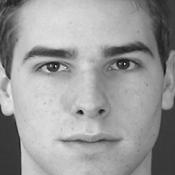
\includegraphics[height=\sz]{Figuras/resultados/E1/E1.png} & 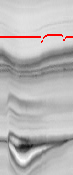
\includegraphics[height=\sz]{Figuras/resultados/E1/E1_YT.png} & 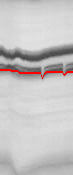
\includegraphics[height=\sz]{Figuras/resultados/E1/E1_XT.png} & 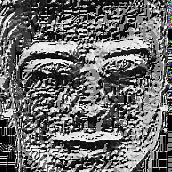
\includegraphics[height=\sz]{Figuras/resultados/E1/E1_LBP.png} & 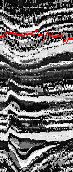
\includegraphics[height=\sz]{Figuras/resultados/E1/E1_LBP_YT.png} & 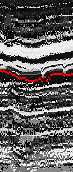
\includegraphics[height=\sz]{Figuras/resultados/E1/E1_LBP_XT.png} \\
		
		\raisebox{.4cm}{\rotatebox{90}{\centering\parbox{2cm}{E2--Asco}}}& 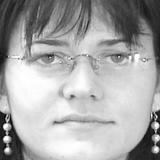
\includegraphics[height=\sz]{Figuras/resultados/E2/E2.png} & 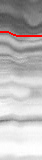
\includegraphics[height=\sz]{Figuras/resultados/E2/E2_YT.png} & 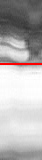
\includegraphics[height=\sz]{Figuras/resultados/E2/E2_XT.png} & 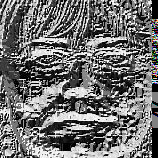
\includegraphics[height=\sz]{Figuras/resultados/E2/E2_LBP.png} & 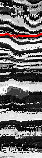
\includegraphics[height=\sz]{Figuras/resultados/E2/E2_LBP_YT.png} & 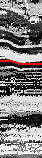
\includegraphics[height=\sz]{Figuras/resultados/E2/E2_LBP_XT.png} \\
		
		\raisebox{.3cm}{\rotatebox{90}{\centering\parbox{2cm}{E3--Miedo}}}& 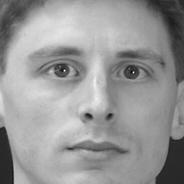
\includegraphics[height=\sz]{Figuras/resultados/E3/E3.png} & 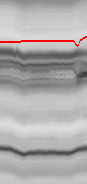
\includegraphics[height=\sz]{Figuras/resultados/E3/E3_YT.png} & 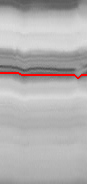
\includegraphics[height=\sz]{Figuras/resultados/E3/E3_XT.png} & 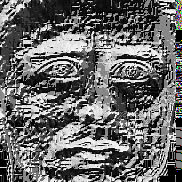
\includegraphics[height=\sz]{Figuras/resultados/E3/E3_LBP.png} & 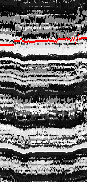
\includegraphics[height=\sz]{Figuras/resultados/E3/E3_LBP_YT.png} & 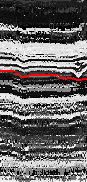
\includegraphics[height=\sz]{Figuras/resultados/E3/E3_LBP_XT.png} \\
		
		\raisebox{.2cm}{\rotatebox{90}{\centering\parbox{2cm}{E4--Alegría}}}& 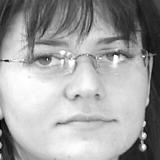
\includegraphics[height=\sz]{Figuras/resultados/E4/E4.png} & 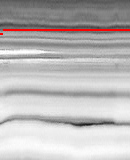
\includegraphics[height=\sz]{Figuras/resultados/E4/E4_YT.png} & 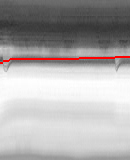
\includegraphics[height=\sz]{Figuras/resultados/E4/E4_XT.png} & 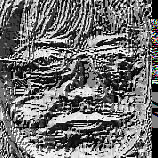
\includegraphics[height=\sz]{Figuras/resultados/E4/E4_LBP.png} & 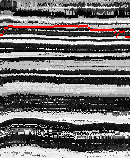
\includegraphics[height=\sz]{Figuras/resultados/E4/E4_LBP_YT.png} & 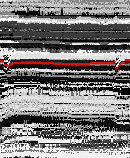
\includegraphics[height=\sz]{Figuras/resultados/E4/E4_LBP_XT.png} \\
		
		\raisebox{0cm}{\rotatebox{90}{\centering\parbox{2cm}{E5--Tristeza}}}& 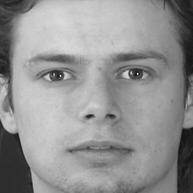
\includegraphics[height=\sz]{Figuras/resultados/E5/E5.png} & 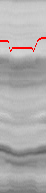
\includegraphics[height=\sz]{Figuras/resultados/E5/E5_YT.png} & 
\includegraphics[height=\sz]{Figuras/resultados/E5/E5_XT.png} & 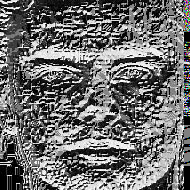
\includegraphics[height=\sz]{Figuras/resultados/E5/E5_LBP.png} & 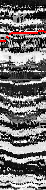
\includegraphics[height=\sz]{Figuras/resultados/E5/E5_LBP_YT.png} & 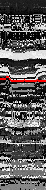
\includegraphics[height=\sz]{Figuras/resultados/E5/E5_LBP_XT.png} \\
		
		\raisebox{0cm}{\rotatebox{90}{\centering\parbox{2.1cm}{E6--Sorpresa}}}& 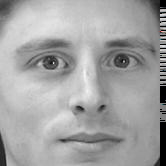
\includegraphics[height=\sz]{Figuras/resultados/E6/E6.png} & 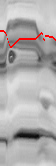
\includegraphics[height=\sz]{Figuras/resultados/E6/E6_YT.png} & 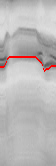
\includegraphics[height=\sz]{Figuras/resultados/E6/E6_XT.png} & 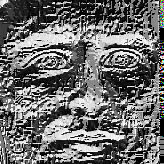
\includegraphics[height=\sz]{Figuras/resultados/E6/E6_LBP.png} & 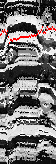
\includegraphics[height=\sz]{Figuras/resultados/E6/E6_LBP_YT.png} & 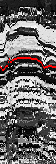
\includegraphics[height=\sz]{Figuras/resultados/E6/E6_LBP_XT.png} \\
		& (a) & (b) & (c) & (d) & (e) & (f) \\

		
	\end{tabular}
	\caption{Tabla comparativa de la extracción de micro-decriptores con vídeos codificados con LBP y sin codificar. Cada fila representa una expresión facial distinta. Las columnas (a) y (d) son el primer cuadro del vídeo, (b) y (e) representan el plano XT, y (c) y (f) representan el plano YT. }
	\label{tabla:comparacion_rayos}
\end{table}


\subsection{Extracción de micro-descriptores}
\label{exp:micro-descriptores}

La extracción de micro-descriptores, etapa propuesta en al Sección~\ref{algoritmo:ext_rayos}, consiste en modelar el movimiento de cada uno de los píxeles a lo largo de todo el vídeo, este modelado es llamado \textit{rayo de flujo}. Para poder extraer un \textit{rayo} se utilizan dos ventanas: la región de soporte y la ventana de búsqueda. Estas regiones permiten calcular a que píxel $(x',y')$ en un tiempo $t+1$ se desplazo el píxel $(x,y)$ en un tiempo $t$. Al de calcular el movimiento de un píxel de $t$ a $t+1$ se crea un \textit{rayo de soporte}, que es el componente mínimo para la creación de los \textit{rayos de flujo}. Para más detalle revisar la Sección~\ref{algoritmo:ext_rayos}.

Para poder evaluar el real modelado de los \textit{rayos} sobre el movimiento de los pixeles, se realizó una extracción de los planos $XT$ y $YT$ del vídeo. El plano $XT$ es una imagen extraída del video en un píxel $(x,y)$, donde cada columna representa un cuadro distinto, donde cada una de estas son extraídas de sus respectivos cuadros $t$, de tal forma que la columna $t$ del plano $XT$ es la fila $y$ del cuadro $t$ del vídeo. Así mismo el plano $YT$ es otra imagen extraída del vídeo en el mismo píxel $(x,y)$, donde cada columna $t$ de este plano representa un cuadro distinto del vídeo, de tal forma que la columna $t$ del plano $YT$ es la columna $x$ del cuadro $t$ del vídeo. Luego de realizar la extracción de los planos y con la posterior obtención del \textit{rayo de flujo} para el pixel $(x,y)$, fue posible realizar un trazado del movimiento del \textit{rayo} en cada una de sus componentes (En el plano $XT$ se trazo el movimiento de la variable $x$ durante los cuadros del vídeo, por el contrario, en el plano $YT$ se trazó el movimiento de la variable $y$). Ejemplos de estos planos y sus trazos pueden ser vistos en la Tabla~\ref{tabla:comparacion_rayos}, en las columnas (b), (c), (e) y (f).

En general revisando los resultados obtenidos en cada uno de los planos, podemos deducir de forma visual que los \textit{rayos de flujo} modelan de forma aproximada el movimiento de los pixeles. Observando la Tabla~\ref{tabla:comparacion_rayos}, nos dimos cuenta que el modelado de los \textit{rayos} no tiene una mayor variación con respecto a la expresión facial que se está observando. Al momento de observar las diferencias entre los resultados obtenidos con los videos con codificación LBP y sin ésta, pudimos observar que los \textit{rayos} obtenidos en vídeos sin LBP obtenían una mejor aproximación al movimiento real del rayo, este comportamiento puede ser observado al comparar la columna (b) y (e) que representa la extracción en el plano $XT$, o comparando (c) y (f) representantes del plano $YT$ en la Tabla~\ref{tabla:comparacion_rayos}. A su vez, se puede observar que las componentes de los \textit{rayos} se comportan mejor al modelar los movimientos verticales (Plano $YT$) que los movimientos horizontales (Plano $XT$), un ejemplo de esto puede ser visto en la expresión (E6), en esta expresión el modelado del movimiento horizontal tiene una aproximación muy baja con respecto a las texturas que se pueden observar en el fondo de la imagen, siendo este un mal modelado de la componente $XT$, por el contrario en la componente del plano $YT$ (columna (c)) se puede observar un modelado casi perfecto con las texturas del fondo de la imagen. Este fenómeno también es visto en otras investigaciones del reconocimiento de expresiones faciales. Ji y Idrissi~\cite{Ji2012} crearon un descriptor espacio temporal que solo utiliza la componente horizontal de los vídeos, ellos se basan en la premisa de que los movimientos significativos del rostro humano tienen una mayor tendencia a ser de forma  vertical que horizontal.

\begin{table}[tb]
	\centering
	\begin{tabular}{ >{\centering\arraybackslash}m{2.5cm}  >{\centering\arraybackslash}m{1.2cm}  >{\centering\arraybackslash}m{1.2cm}  >{\centering\arraybackslash}m{1.2cm}  >{\centering\arraybackslash}m{1.2cm}  >{\centering\arraybackslash}m{1.2cm}  >{\centering\arraybackslash}m{1.2cm} }
		\hline
		Codificación & \multicolumn{3}{ c }{XT} & \multicolumn{3}{ c }{YT}\\
		\hline
		& & & & & &\\
		Sin codificación & 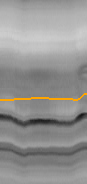
\includegraphics[width=1.2cm]{Figuras/resultados/comparacion_real/no_lbp/YT/extraido.png} & 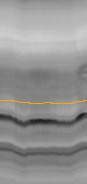
\includegraphics[width=1.2cm]{Figuras/resultados/comparacion_real/no_lbp/YT/pintado.png} & 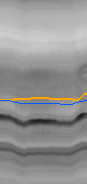
\includegraphics[width=1.2cm]{Figuras/resultados/comparacion_real/no_lbp/YT/superposicion.png} & 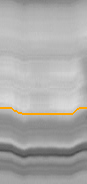
\includegraphics[width=1.2cm]{Figuras/resultados/comparacion_real/no_lbp/XT/extraido.png} & 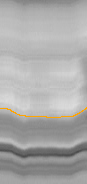
\includegraphics[width=1.2cm]{Figuras/resultados/comparacion_real/no_lbp/XT/pintado.png} & 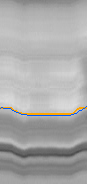
\includegraphics[width=1.2cm]{Figuras/resultados/comparacion_real/no_lbp/XT/superposicion.png} \\
		
		Codificación LBP & 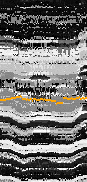
\includegraphics[width=1.2cm]{Figuras/resultados/comparacion_real/lbp/YT/extraido.png} & 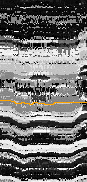
\includegraphics[width=1.2cm]{Figuras/resultados/comparacion_real/lbp/YT/pintado.png} & 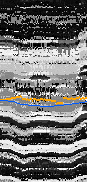
\includegraphics[width=1.2cm]{Figuras/resultados/comparacion_real/lbp/YT/superposicion.png} & 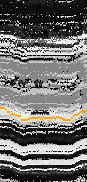
\includegraphics[width=1.2cm]{Figuras/resultados/comparacion_real/lbp/XT/extraido.png} & 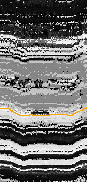
\includegraphics[width=1.2cm]{Figuras/resultados/comparacion_real/lbp/XT/pintado.png} & 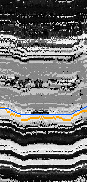
\includegraphics[width=1.2cm]{Figuras/resultados/comparacion_real/lbp/XT/superposicion.png} \\

		& (i) & (ii) & (iii) & (iv) & (v) & (vi)\\

	\end{tabular}
	\caption{Tabla comparativa de el calculo del error de cada plano. (i) y (iv) representan el \textit{rayo} extraído por el algoritmo; (ii) y (v) el \textit{rayo} promedio dibujado por las personas; (iii) y (vi) la superposición de ambos (de color amarillo el extraído y color azul el promedio). }
	\label{tabla:comparacion_errores}
\end{table}


Para poder ratificar las observaciones que hemos podido deducir al contemplar el movimiento a través de los planos, se diseñó un experimento que nos permitió calcular un error aproximado del modelado de los \textit{rayos de flujo}. Este experimento consistió en pedir a distintas personas que dibujaran el \textit{rayo de flujo} sobre cada plano, para esto utilizaron la herramienta de dibujo paint de Windows. En general se pidió a cada una de las personas que dibujaran como creían ellos que se movía el pixel inicial a lo largo de las texturas representadas en el plano. Luego de esta etapa se procedió a extraer cada una de las componentes de los \textit{rayos} dibujados a mano, con esto se logró calcular un promedio de los trazos de las personas. Este \textit{rayo} promedio es comparado con el extraído por el algoritmo, de tal forma que se puede calcular el error para cada componente y un error general. Este proceso puede ser visualizado en la Tabla~\ref{tabla:comparacion_errores}, donde las columnas (iii) y (iv), representan de forma visual como se superpone un \textit{rayo} sobre otro. El error es obtenido calculando la desviación estándar entre ambas componentes. 

\pgfplotstableset{
  franjas/.style={
    columns/errorG/.style={
      column name=Error,
      precision=1
    },
    every even row/.style={
      before row={\rowcolor{#1}}
    },
    every head row/.style={
      before row=\hline\noalign{\smallskip},after row=\hline
    },
    every last row/.style={
      after row=\hline
    },
  },
  franjas/.default={gray!50},
  tablita/.style={
    columns={rs, ws, errorYT, errorXT, errorG},
    columns/rs/.style={
      column name=$RS$,
    },
    columns/ws/.style={
      column name=$WS$,
    },
    columns/errorXT/.style={
      column name=Error $YT$,
      precision=1
    },
    columns/errorYT/.style={
      column name=Error $XT$,
      precision=1
    },
    franjas,
  },
  tablaK/.style={
  	columns={N, K, Accuracy},
  	columns/N/.style={
  		column name=$N$,
  	},
  	columns/K/.style={
  		column name=$K$,
  	},
  	columns/Accuracy/.style={
  		column name=Accuracy,
  		precision=1,
  		postproc cell content/.append style={
  			/pgfplots/table/@cell content/.add={}{\,\%}
  		}
  	},
  	franjas,
  },
  tablaN/.style={
  	columns={RS, WS, N, Accuracy},
  	columns/RS/.style={
  		column name=$RS$,
  	},
  	columns/WS/.style={
  		column name=$WS$,
  	},
  	columns/N/.style={
  		column name=$N$,
  	},
  	columns/Accuracy/.style={
  		column name=Accuracy,
  		precision=1,
  		postproc cell content/.append style={
  			/pgfplots/table/@cell content/.add={}{\,\%}
  		}
  	},
  	franjas,
  },
  tablaSVMresultsRBF/.style={
  	columns={Gamma,C-value,Accuracy},
  	columns/Gamma/.style={
  		column name=$Gamma$,
  		precision=3
  	},
  	columns/C-value/.style={
  		column name=$C-value$,
  		precision=3
  	},
  	columns/Accuracy/.style={
  		column name=$Accuracy$,
  		precision=1,
  		postproc cell content/.append style={
  			/pgfplots/table/@cell content/.add={}{\,\%}
  		}
  	},
  	franjas,
  },
  tablaSVMresultsLineal/.style={
  	columns={C-value,Accuracy},
  	columns/C-value/.style={
  		column name=$C-value$,
  		precision=3
  	},
  	columns/Accuracy/.style={
  		column name=$Accuracy$,
  		precision=1,
  		postproc cell content/.append style={
  			/pgfplots/table/@cell content/.add={}{\,\%}
  		}
  	},
  	franjas,
  },
  tablaSVMresultsPoly/.style={
  	columns={Degree,Gamma,C-value,Accuracy},
  	columns/Degree/.style={
  		column name=$Degree$,
  	},
  	columns/Gamma/.style={
  		column name=$Gamma$,
  		precision=3
  	},
  	columns/C-value/.style={
  		column name=$C-value$,
  		precision=3
  	},
  	columns/Accuracy/.style={
  		column name=$Accuracy$,
  		precision=1,
  		postproc cell content/.append style={
  			/pgfplots/table/@cell content/.add={}{\,\%}
  		}
  	},
  	franjas,
  },
  tablaSVMresults/.style={
  	columns={RS,WS,N,K,Accuracy},
  	columns/RS/.style={
  		column name=$RS$,
  	},
  	columns/WS/.style={
  		column name=$WS$,
  	},
  	columns/N/.style={
  		column name=$N$,
  	},
  	columns/K/.style={
  		column name=$K$,
  	},
  	columns/Accuracy/.style={
  		column name=$Accuracy$,
  		precision=1,
  		postproc cell content/.append style={
  			/pgfplots/table/@cell content/.add={}{\,\%}
  		}
  	},
  	franjas,
  },
  tablaSVMresultscmp/.style={
	  columns={Autor,K-fold,Accuracy},
	  columns/Accuracy/.style={
	  	column name=$Accuracy$,
	  	precision=1,
	  	postproc cell content/.append style={
	  		/pgfplots/table/@cell content/.add={}{\,\%}
	  	}
	  },
	  franjas,
	},
}

\begin{table}[tb]
	\centering
	\pgfplotstabletypeset[tablita]{Datos/comparacion_NO_LBP.dat}
	\caption{Tabla comparativa de los errores encontrados en los planos $XT$, $YT$ y error general, al calcular los \textit{rayos} con distintos tamaños de ventanas. Sin codificación LBP.}
	\label{tabla:error_no_lbp}
\end{table}

\begin{table}[tb]
	\centering
	\pgfplotstabletypeset[tablita]{Datos/comparacion_LBP.dat}
	\caption{Tabla comparativa de los errores encontrados en los planos $XT$, $YT$ y error general, al calcular los \textit{rayos} con distintos tamaños de ventanas. Con codificación LBP.}
	\label{tabla:error_lbp}
\end{table}

Decidimos utilizar esta métrica de comparación para visualizar cómo se comportan los \textit{rayos} con respecto al tamaño de las ventanas utilizadas. En las Tablas~\ref{tabla:error_no_lbp}~y~\ref{tabla:error_lbp} se puede ver reflejados los cálculos resultantes del error en ambos planos y el error general calculado como el promedio entre ambos errores, utilizando distintos tamaños de ventanas. Con estos resultados logramos darnos cuenta que la idea planteada sobre las diferencias del modelado vertical y horizontal estaba en lo cierto, en ambas tablas podemos ver que el error obtenido en el plano $YT$ es mucho menor al obtenido en $XT$. Además en general los errores disminuyen a medida que se aumenta el tamaño de las ventanas $RS$ y $WS$, esto es debido a que mientras más grande sea la región de soporte, menos probabilidad existe de encontrar otra textura igual en la imagen, por lo cual la probabilidad de encontrar en el siguiente cuadro el movimiento de la misma textura es mucho más alta.

\begin{figure}[t]
	\begin{subfigure}{1.0\textwidth}
		\centering
		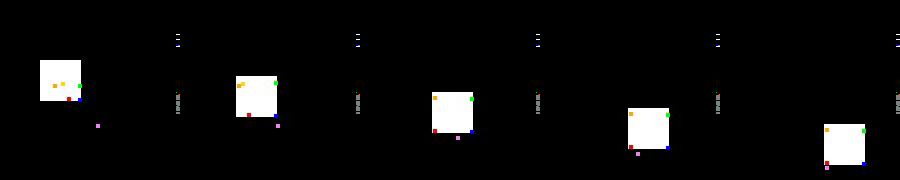
\includegraphics[width=1\textwidth]{Figuras/resultados/videos_sinteticos/v1.png}
		\caption{Vídeo sintético simple sin texturas}
		\label{exp:fig:vs1}
	\end{subfigure}
	
	\begin{subfigure}{1.0\textwidth}
		\centering
		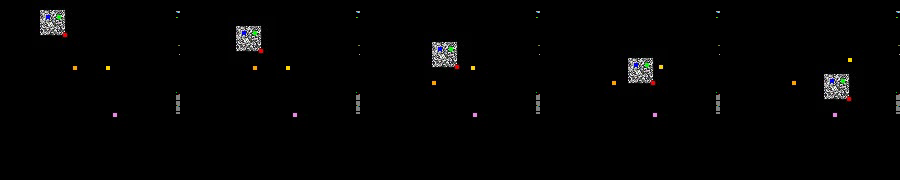
\includegraphics[width=1\textwidth]{Figuras/resultados/videos_sinteticos/v2.png}
		\caption{Vídeo sintético simple con texturas}
		\label{exp:fig:vs2}
	\end{subfigure}
	
	\begin{subfigure}{1.0\textwidth}
		\centering
		\includegraphics[width=1\textwidth]{Figuras/resultados/videos_sinteticos/v3.png}
		\caption{Vídeo sintético con texturas.}
		\label{exp:fig:vs3}
	\end{subfigure}
	\caption{Cortes de vídeos sintéticos, en los cuales se describe el movimiento de ciertos pixeles a lo largo del tiempo.} 
	\label{exp:fig:vs}
\end{figure}

Luego de obtener resultados satisfactorios con el modelado de los \textit{rayos de flujo}, decidimos probar si la teoría de extracción de éstos podía ser aplicada a otros vídeos y otras texturas, por lo que preparamos un conjunto de vídeos sintéticos, los cuales describían movimientos predecibles al ojo humano. En estos vídeos se representó el movimiento de regiones cuadradas con y sin textura, y también se generó un video que permitió examinar que sucede con los rayos si existen dos movimientos distintos.

Luego de realizar la extracción de \textit{rayos de flujo} a los vídeos generados sintéticamente, observamos dos fenómenos. Los rayos pueden modelar el movimiento de los pixeles a los largo del tiempo, esto puede ser visto en la Figura~\ref{exp:fig:vs}, en la cual se ven cortes de distintos cuadros de los vídeos y como se mueven los pixeles escogidos, estos pixeles son representados con cuadros de color a lo largo del vídeo. También descubrimos que el modelado de los \textit{rayos} tiene un comportamiento más estable cuando existen texturas en las zonas que se están analizando, como se puede ver en las Figuras~\ref{exp:fig:vs2}~y~\ref{exp:fig:vs3}, los píxeles internos del cuadrado siguen durante todo el movimiento en la misma posición del cuadrado, no así en la Figura~\ref{exp:fig:vs1}, en la cual los pixeles que están dentro del cuadrado tienden a juntarse en un punto a medida que el cuadrado se va desplazando. 

En general, por lo que pudimos apreciar en el desarrollo de todos estos experimentos, el comportamiento de los \textit{rayos} depende de dos componentes claves para conseguir un buen modelado, primero una elección inteligente del tamaño de las ventanas $RS$ y $WS$, esto debido a que una ventana más grande disminuye las probabilidades de error a la hora de elegir el movimiento del pixel, pero a su vez aumenta el costo computacional del algoritmo, debido a que se deben realizar mas cálculos a la hora de la elección del movimiento; segundo, otra componente clave es el nivel de detalle de la textura abarcada por las ventanas, esto debido a que una textura plana puede ser fácilmente confundida con otra textura plana similar, a su vez una textura con detalle permite que el modelado sea más real con respecto a los reales movimientos del rostro humano. 

\subsection{ Normalización de micro-descriptores }

Luego de concretar la extracción de los micro-descriptores, se procedió a realizar una normalización de los \textit{rayos de flujo}, ésta consistió en poder realizar una reducción o ampliación de los rayos, esto con el fin de que todos los micro-descriptores tengan el mismo largo $N$, ésto nos permitió tener a todos los \textit{rayos} en el mismo espacio vectorial. Para detalles sobre esta etapa revisar la Sección~\ref{algoritmo:normalizacion}.
\begin{table}[Bt]
	\centering
	\pgfplotstabletypeset[tablaN]{Figuras/resultados/Normalizacion/Accuracy_n.dat}
	\caption{Tabla comparativa de la Asertividad o \textit{Accuracy} (en ingles) obtenido utilizando distintos valores de $N$ y distintos tamaños de las ventanas.}
	\label{tabla:accuracy_N}
\end{table}

Para poder evaluar que valores de la variable $N$ escoger al momento de realizar la normalización, se decidió realizar una comparación entre el valor de la variable $N$ y la asertividad o \textit{Accuracy} reconociendo las expresiones faciales. Estos resultados pueden ser vistos en la Tabla~\ref{tabla:accuracy_N}, para obtener resultados se utilizaron valores de las ventanas $RS$ y $WS$ estudiados en la Sección~\ref{exp:micro-descriptores}. 

Observando los resultados logramos deducir que no existe una gran variación en el \textit{Accuracy} con respecto a los valores de la normalización. En general observamos que el comportamiento de la asertividad no tenía una dependencia muy directa del tamaño de la normalización, esto debido a que este procedimiento lo único que hace es realizar proyección lineal del espacio vectorial sobre un nuevo espacio parametrizado por la variable $N$, visto desde la parte matemática, este procedimiento además de ayudar a poder comparar vectores de distintas dimensiones, permitió realizar una transformación de cada uno de estos \textit{rayos} a un espacio vectorial común para su posterior agrupamiento. 



\subsection{ Creación de macro-descriptores }

La creación de los macro-descriptores es la etapa final de la extracción de características de los vídeos, se utilizó la técnica \textit{Bag of visual words} analizada en la Sección~\ref{sec:bag_of_words}, para obtener un diccionario que permita representar el espacio vectorial a analizar, en el caso de nuestra implementación es necesario obtener un conjunto de \textit{rayos de flujo} representativos del espacio, este conjunto es llamado vocabulario, y en el se encuentran todas las posibles palabras que pueden existir en el universo formado por los datos de entradas. Para poder obtener este vocabulario sobre nuestros micro-descriptores, se utilizó la técnica de agrupamiento no supervisada $k$-means analizada en la Seccion~\ref{sec:k-means}, la cual recibe como entrada un grupo de vectores (\textit{rayos de flujo}) y la cantidad $K$ de grupos a formar, con esto calcula cada uno de los vectores o \textit{rayos} representantes, los cuales son el vocabulario utilizado por el \textit{Bag of visual words}. Luego de obtener este vocabulario, se procede a construir los macro-descriptores de cada vídeo, calculando un histograma de tamaño $K$, el cual es la representación de la frecuencia de asociación de cada \textit{rayo} con su respectivo \textit{cluster} $k$. Para más detalles de esta etapa revisar la Sección~\ref{sec:macro-descriptores}. Con esto logramos deducir que la variable $K$, es de suma importancia para el algoritmo, esto debido a que la construcción de los descriptores finales de cada vídeo dependen del valor asignado a esta variable.

\newlength{\st}
\setlength{\st}{1.5cm}
\setlength{\sz}{1.6cm}
\begin{table}[tb]
	\centering
	\begin{tabular}{ >{\centering\arraybackslash}m{.5cm}  >{\centering\arraybackslash}m{\st}  >{\centering\arraybackslash}m{\st}  >{\centering\arraybackslash}m{\st}  >{\centering\arraybackslash}m{\st}  >{\centering\arraybackslash}m{\st}  >{\centering\arraybackslash}m{\st}  }
		\hline\noalign{\smallskip}
		$K$ & Ira & Asco & Miedo & Alegría & Tristeza & Sorpresa\\
		\hline\noalign{\smallskip}
		10 & \includegraphics[height=\sz]{Figuras/resultados/clustering/k=10/E1_ec.png} & \includegraphics[height=\sz]{Figuras/resultados/clustering/k=10/E2_ec.png} & \includegraphics[height=\sz]{Figuras/resultados/clustering/k=10/E3_ec.png} & \includegraphics[height=\sz]{Figuras/resultados/clustering/k=10/E4_ec.png} & \includegraphics[height=\sz]{Figuras/resultados/clustering/k=10/E5_ec.png} & \includegraphics[height=\sz]{Figuras/resultados/clustering/k=10/E6_ec.png} \\
		
		50 & \includegraphics[height=\sz]{Figuras/resultados/clustering/k=50/E1_ec.png} & \includegraphics[height=\sz]{Figuras/resultados/clustering/k=50/E2_ec.png} & \includegraphics[height=\sz]{Figuras/resultados/clustering/k=50/E3_ec.png} & \includegraphics[height=\sz]{Figuras/resultados/clustering/k=50/E4_ec.png} & \includegraphics[height=\sz]{Figuras/resultados/clustering/k=50/E5_ec.png} & \includegraphics[height=\sz]{Figuras/resultados/clustering/k=50/E6_ec.png} \\
		
		100 & \includegraphics[height=\sz]{Figuras/resultados/clustering/k=100/E1_ec.png} & \includegraphics[height=\sz]{Figuras/resultados/clustering/k=100/E2_ec.png} & \includegraphics[height=\sz]{Figuras/resultados/clustering/k=100/E3_ec.png} & \includegraphics[height=\sz]{Figuras/resultados/clustering/k=100/E4_ec.png} & \includegraphics[height=\sz]{Figuras/resultados/clustering/k=100/E5_ec.png} & \includegraphics[height=\sz]{Figuras/resultados/clustering/k=100/E6_ec.png} \\
		
		500 & \includegraphics[height=\sz]{Figuras/resultados/clustering/k=500/E1_ec.png} & \includegraphics[height=\sz]{Figuras/resultados/clustering/k=500/E2_ec.png} & \includegraphics[height=\sz]{Figuras/resultados/clustering/k=500/E3_ec.png} & \includegraphics[height=\sz]{Figuras/resultados/clustering/k=500/E4_ec.png} & \includegraphics[height=\sz]{Figuras/resultados/clustering/k=500/E5_ec.png} & \includegraphics[height=\sz]{Figuras/resultados/clustering/k=500/E6_ec.png} \\
		
		1000 & \includegraphics[height=\sz]{Figuras/resultados/clustering/k=1000/E1_ec.png} & \includegraphics[height=\sz]{Figuras/resultados/clustering/k=1000/E2_ec.png} & \includegraphics[height=\sz]{Figuras/resultados/clustering/k=1000/E3_ec.png} & \includegraphics[height=\sz]{Figuras/resultados/clustering/k=1000/E4_ec.png} & \includegraphics[height=\sz]{Figuras/resultados/clustering/k=1000/E5_ec.png} & \includegraphics[height=\sz]{Figuras/resultados/clustering/k=1000/E6_ec.png} \\
		
		& (E1) & (E2) & (E3) & (E4) & (E5) & (E6) \\
	\end{tabular}
	\caption{Tabla comparativa de la cantidad de \textit{cluster} utilizados y su representación en las distintas expresiones faciales. Las imágenes fueron construidas en escala de grises, los colores mas cercanos al blanco representan mayor cantidad de \textit{rayos} agrupados en ese conjunto. }
	\label{tabla:comparacion_clusters} 
\end{table}	

\begin{table}[tb]
	\centering
	\pgfplotstabletypeset[tablaK]{Figuras/resultados/clustering/Accuracy_k.dat}
	\caption{Tabla comparativa de la Asertividad o \textit{Accuracy} (en ingles) obtenido utilizando distintos valores de $K$.}
	\label{tabla:accuracy_K}
\end{table}

Para poder evaluar si esta técnica realizó un modelado exitoso preparamos dos experimentos, el primero consistió en poder realizar una evaluación visual del movimiento de los grupos o \textit{clusters} de \textit{rayos}, siendo éstos representados sobre el rostro que fue analizado. En general sabemos por la extracción de \textit{rayos de flujo}, que cada uno de estos tiene asociada una posición inicial dentro del rostro analizado, con lo cual se procedió a crear imágenes en escala de grises, las cuales representan los \textit{clusters} dentro del vídeo. Algunos ejemplos pueden ser vistos en la Tabla~\ref{tabla:comparacion_clusters}. 

Las imágenes fueron construidas calculando y ordenando los $P$ grupos con mayor frecuencia ( 0 <\ $P$ <\ 255 y $P \leq K$ ), cada grupo $p$ fue asignado a un valor en la escala de grises, a los grupos que obtuvieron una mayor frecuencia de aparición les fueron asignado valores más cercanos a $255$ (Color blanco), del mismo modo los \textit{clusters} con menor frecuencia obtienen valores más cercanos a $0$ (Color negro), a su vez todos los demás grupos que quedaron fuera de la selección inicial reciben el valor $0$. Esto debido a que los \textit{cluster} con menor frecuencia pueden ser catalogados como \textit{rayos} ruidosos, y que no aportan información al sistema.

Observando las imágenes obtenidas y representadas en la Tabla~\ref{tabla:comparacion_clusters}, logramos percatarnos que existe una gran segmentación de las regiones más importantes del rostro (Ojos, cejas, nariz y boca). A medida que la variable $K$ aumenta, logramos visualizar de mejor manera las regiones de interés. El ejemplo más característico puede ser visualizado en la expresión de sorpresa (E6), cuando $K$ tomó el valor 10, en (E6) observamos una tendencia de los \textit{clusters} a agruparse en las regiones importantes, conforme fue aumentando el valor de $K$, la imagen del rostro se fue volviendo mas nítida llegando a detectar visualmente de forma muy directa las partes importantes del rostro (véase la secuencia de imágenes de (E6) con distintos valores $K$), así mismo esto paso con el general de los vídeos utilizados en los experimentos. También logramos deducir que visualmente no existe una dependencia entre la expresión facial que se quiso representar y las regiones del rostro más nítidas.

Cabe destacar que por las observaciones realizadas, es de vital importancia una elección inteligente de la cantidad de grupos a crear, esto debido a que un valor muy pequeño puede hacer que los conjuntos encontrados estén muy poco segmentados (Ver $K$ = 10 en la Tabla~\ref{tabla:comparacion_clusters}), por el contrario un valor muy alto puede provocar una sobre segmentación de los \textit{cluster}, de tal forma que los \textit{rayos} estén tan segmentados que los clasificadores no puedan encontrar patrones en los macro-descriptores de la misma expresión.

El segundo experimento consistió en buscar de forma mas empírica un valor que permita la creación de un buen modelo de clasificación a la hora de etiquetar nuevas expresiones entrantes. Para esto se realizó una comparación de distintos valores $K$ y su asertividad a la hora de clasificar. Estos resultados son expuestos en la Tabla~\ref{tabla:accuracy_K}, y fueron obtenidos al utilizar los mejores valores resultantes en las variables analizadas en las secciones anteriores de este capítulo, los resultados obtenidos son bastante pobres a pesar de los cambios de la variable $K$, esto puede ser debido a un mal agrupamiento por parte del algoritmo. Es de vital importancia mencionar que los algoritmos de \textit{clustering} son muy sensibles a las semillas ingresadas como puntos iniciales, para estos experimentos utilizamos un algoritmo de elección inteligente de las semillas, este método esta basado en las investigaciones de Arthur y Vassilvitskii~\cite{Arthur2007}, el cual esta implementado en la librería OpenCV.

En general, luego de observar los resultados de los experimentos expuestos, podemos visualizar una necesidad de seguir profundizando en el tema de como construir los macro-descriptores, proponemos realizar investigaciones sobre los distintos algoritmos que se pueden utilizar a la hora de agrupar, revisar cuales medidas de distancia permiten un mejor agrupamiento de los \textit{rayos}, buscar como inicializar de mejor manera las semillas. Por otra parte revisando los resultados obtenidos al realizar el mapeo de los \textit{clusters} en el rostro proponemos realizar una extracción de los \textit{rayos de flujo} solo sobre las regiones importantes del rostro, ya que creemos que al no extraer los \textit{rayos} de las regiones que aportan ruido, los macro-descriptores resultantes tendrán mas patrones que permitirán mejores resultados a la hora de clasificar. 

\subsection{ Entrenamiento y clasificación }


\begin{table}[b]
	\centering
	\pgfplotstabletypeset[tablaSVMresultsRBF]{Datos/rbf_10.csv}
	\caption{Mejores resultados obtenidos por el Kernel RBF.}
	\label{tabla:svm_rbf}
\end{table}
\begin{table}[tb]
	\centering
	\pgfplotstabletypeset[tablaSVMresultsLineal]{Datos/lineal_10.csv}
	\caption{Mejores resultados obtenidos por el Kernel Lineal.}
	\label{tabla:svm_lineal}
\end{table}
\begin{table}[tb]
	\centering
	\pgfplotstabletypeset[tablaSVMresultsPoly]{Datos/poly_10.csv}
	\caption{Mejores resultados obtenidos por el Kernel Polinomial.}
	\label{tabla:svm_poly}
\end{table}

El entrenamiento y clasificación es de vital importancia, debido a que en esta etapa es cuando se genera el modelo que permite clasificar las nuevas expresiones entrantes. Este modulo puede ser dividido en dos partes, primero el entrenamiento, el cual es el encargado de encontrar un modelo que permita clasificar de la mejor forma las nuevas entradas; segundo la clasificación, etapa encargada de etiqueta con alguna expresión las nuevas entradas, esta etiqueta es asignada dependiendo del modelo entrenado en la fase anterior. También en esta etapa se realiza el cálculo de la asertividad o \textit{Accuracy} del algoritmo. Para obtener un cálculo más real del modelo generado se utilizó la técnica de $k$-fold~cross-validation, la cual en simples palabras consiste en separar los datos de forma aleatoria en dos grupos (Entrenamiento y pruebas), realizando esta separación $k$ veces y para cada una de estas separaciones obteniendo un \textit{Accuracy} el cual es el promediado de todas separaciones, este promedio es el promedio que se utiliza como medida de comparación. Para todos los experimentos expuestos en esta Sección se utilizó un 10-fold~cross-validación y SVM. Para mayores detalles de esta etapa, revisar la Sección~\ref{sec:clasificacion}.

Como se explico en la Sección~\ref{sec:svm}, SVM trata de encontrar una recta que permita separar a los dos grupos datos dentro de un mismo espacio vectorial, en el general de los casos reales no existe una recta que permita separar de forma efectiva ambas clases, por esto SVM hace uso de las técnicas de Kernel, en simples palabras estas técnicas permiten realizar transformación lineales de los espacios vectoriales, con lo cual se puede realizar la búsqueda de un hiper-plano que logre segmentar ambas clases y minimice el error. Debido a esto realizamos un experimento que permita encontrar de forma empírica cual de los Kernel y valores de sus respectivas variables maximicen el \textit{Accuracy}, Los Kernels utilizados están implementados en la librería en OpenCV la cual se basa LibSVM creada por Chang~y~Lin~\cite{Chang2011} para obtener resultados de SVM.


Como podemos observar en las Tablas~\ref{tabla:svm_rbf},~\ref{tabla:svm_lineal}~y~\ref{tabla:svm_poly}, se obtuvieron resultados muy bajos, y en general no existe mucha variación entre la utilización de un kernel u otro. La Tabla~\ref{tabla:svm_lineal} contiene los mejores valores obtenidos en los experimentos al utilizar un kernel lineal, en simples palabras este kernel no realiza ninguna transformación lineal sobre el espacio, por lo cual la única variable que utiliza es la penalización por una mala clasificación, llamada C-$value$. En general al variar con distintos valores para la penalización no se obtuvieron grandes cambios en el \textit{Accuracy} del modelo. De la misma forma como podemos visualizar en la Tabla~\ref{tabla:svm_poly}, los resultados obtenidos por el kernel polinomial no demuestran un cambio radical con respecto a la variación de los valores de las variables, siendo estas el valor de penalización (C-$value$), el grado del polinomio ($Degree$), el cual indica el grado polinomial del espacio a transformar y por ultimo la variable de suavizado ($\gamma$). Por ultimo al revisar los resultados expuestos en la Tabla~\ref{tabla:svm_rbf}, los cuales fueron obtenidos por el kernel RBF, el cual permite realizar una transformación a espacios circulares, podemos visualizar que al igual que en las tablas anteriores no existe una variación en los resultados obtenidos al variar los valores de las variables (C-$value$ y $\gamma$). Con estos resultados obtenidos concluimos que en general los resultados obtenidos por los distintos kernels no varían mucho entre si, por lo cual para los experimentos generales del sistema utilizamos un kernel RBF, esto debido a que este kernel permitió obtener los mejores resultados.

%Como se puede observar en las Tablas~\ref{tabla:svm_rbf},~\ref{tabla:svm_lineal}~y~\ref{tabla:svm_poly}, se obtuvieron resultados muy bajos, en general, los mejores \textit{Accuracy} fueron obtenidos utilizando el Kernel RBF, el cual permite realizar una transformación lineal, donde una recta en el espacio del Kernel puede ser representada por una circunferencia en el plano real de los datos. Revisando los valores de las variables ($\gamma$, \textit{Degree} y $C$-value), observamos que no existe una segmentación clara sobre que valores deben adquirir estas variables para obtener mejores resultados a la hora de entrenar el modelo. En la Sección~\ref{sec:svm}, nombramos distintos kernels que podrían ser utilizados para el problema de clasificación, entre ellos \textit{Histogram Intersection}, el cual tiene una gran efectividad a la hora de generar un modelo de vectores representantes de histogramas, este kernel no está incluido en la implementación de SVM en la librería OpenCV. Por lo cual es importante buscar alguna implementan de SVM que tenga incluido este kernel.
\begin{table}[bt]
	\centering
	\pgfplotstabletypeset[tablaSVMresults]{Datos/resultados.dat}
	\caption{Resultados obtenidos utilizando las mejores variables obtenidas en el proceso de experimentos.}
	\label{tabla:exp:accuracy}
\end{table}


Por último como experimento final decidimos realizar una comparación del \textit{Accuracy} obtenido con los mejores valores de las variables del algoritmo ($RS$, $WS$, $N$, $K$). Al visualizar la Tabla~\ref{tabla:exp:accuracy}, podemos darnos cuenta que los mejores valores de  \textit{Accuracy} obtenidos por nuestro método no alcanzan el 49\% de asertividad, lo cual es un valor bastante bajo con respecto a los mejores resultados obtenidos en el estado del arte, dichos resultados pueden ser visualizados la Tabla~\ref{tabla:exp:accuracy_cmp}, en la cual se muestra el \textit{Accuracy} de distintos métodos de reconocimiento de expresiones faciales en video, cuyos valores de asertividad son mayores al al 88\%: Al comparar estos valores con nuestros resultados podemos deducir que nuestro algoritmo no esta obteniendo resultados significativos con respecto a los mejores métodos. Nosotros creemos que estos malos resultados son ocacionados por la cantidad de ruido que es agregado al extraer los \textit{rayos de flujo} de regiones del rostro que no aportan información. 



\begin{table}[tb]
	\centering
	\begin{tabular}{l c}
		\hline
		Autor & \textit{Accuracy}\\
		\hline
		\rowcolor{gray!50} 
		Yeasin~\etal~\cite{Yeasin2004} & 90.0 \% \\
		
		Xiang~\etal~\cite{Xiang2008}& 88.8 \%\\
		
		\rowcolor{gray!50} 
		Buenaposada~\etal~\cite{Buenaposada2008} & 89.1 \%\\
		
		Zhao~y~Pietikäinen~\cite{Zhao2007}~a & 95.1 \%\\
		
		\rowcolor{gray!50} 
		Zhao~y~Pietikäinen~\cite{Zhao2007}~b & 93.8 \%\\
		
		Ji~y~Idrissi~\cite{Ji2012} LBP & 91.6 \%\\
		
		\rowcolor{gray!50} 
		Ji~y~Idrissi~\cite{Ji2012} LBP + VTB & 93.6 \%\\
		
		Ji~y~Idrissi~\cite{Ji2012} Moments & 98.5 \%\\
		
		\rowcolor{gray!50} 
		\textit{Rayos de flujo} & 48.6 \%\\
		\hline
	\end{tabular}
	\caption{Tabla comparativa de resultados obtenidos con distintos métodos en el estado del arte.}
	\label{tabla:exp:accuracy_cmp}
\end{table}




En resumen, luego de ver los resultados obtenidos en todos los experimentos de este capítulo, llegamos a las siguientes conclusiones: la teoría de extracción de \textit{rayos de flujo} logra modelar los movimientos de las texturas a lo largo del tiempo, este modelado es más efectivo al reproducir el movimiento vertical que el horizontal, por lo cual una posible forma de mejorar el método es solo utilizar la componente vertical de los \textit{rayos} o utilizar el angulo de movimiento que es formado por ambas componentes; el modelado de los \textit{rayos} es mucho mas estable en ambas componentes al utilizar regiones $RS$ y $WS$ más grandes, el problema es que mientras mas grande sean las ventanas mayor sera el tiempo computacional de la extracción; vemos una necesidad de realizar una segmentación de las partes importantes del rostro, esto debido a que la extracción de micro-descriptores esta siendo realizada en todos los pixeles de la imagen, lo cual agrega mucha información no necesaria o ruido, por lo cual creemos que es necesario realizar la extracción solo de las partes importantes del rostro como los ojos, la nariz y la boca; el valor de la variable de normalización $N$ no trae grandes cambios a la hora de obtener mejores resultados, pero la utilización de esta variable es de vital importancia, ya que, nos permite realizar las transformaciones de los \textit{rayos} al mismo espacio, por ende estos pueden ser comparados entre si; en general luego de realizar el agrupamiento en la etapa de creación macro-descriptores y realizar la representación de los movimientos del rostro vista en la Tabla~\ref{tabla:comparacion_clusters}, logramos darnos cuenta que el modelado de los \textit{rayos} y posterior agrupamiento tiende a mostrar patrones con respecto a como se mueven las regiones del rostro, siendo las mas sobresalientes las regiones importantes, pero como puede ser visualizado en la tabla, también existe mucho ruido, el cual no permite realizar una agrupación adecuada, por ende es necesario seguir profundizando en la forma de agrupar los \textit{rayos}, esto debido a que el método de agrupamiento propuesto no demuestra tener resultados satisfactorios con respecto al \textit{Accuracy}, esto puede ser por dos motivos, primero el culpable puede ser la extracción de micro-descriptores, esto debido a que se están agregando muchos \textit{rayos} ruidosos al sistema, o segundo, puede ser por una mala agrupación o inicialización por parte del \textit{Bag of Visual Words}.

%Esta comparación puede ser visualizada en la Tabla~\ref{}. 

%En general y al igual que en la mayoría de los experimentos de obtención de \textit{Accuracy}, se obtuvieron resultados muy pobres, esto puede ser debido a una mala aproximación de los valores de las variables de los kernels, o que los kernels que se utilizan no permiten realizar un mapeo exitoso del espacio vectorial observado. Otro posible problema puede ser el tamaño de los conjuntos de entrenamiento y prueba utilizados por el $k$-fold cross validation, debido a que para todos los experimentos se utilizó un 50\% de los videos para el entrenamiento, por lo cual puede existir una necesidad del clasificador por tener más datos de entrenamiento, para así poder obtener un mejor modelo de clasificación.


